\section{Evolution of Massive Stars in Isolation}\label{sec:single_star_evolution}

Stars with $M \leq 2$ M$_{\odot}$, $2 < M \leq 8$ M$_{\odot}$ and $M > 8$ M$_{\odot}$ are classified as low-, intermediate-, and high-mass, respectively. Despite the inherent rarity predicted by the initial mass function (IMF, see e.g. \cite{chabrier2005initial, dib2018emergence}), massive stars play a key role in the evolution of the Universe. They are the main source of UV radiation and heavy elements. They serve as a significant source of mixing and turbulence in the interstellar medium (ISM) of galaxies through a combination of winds, outflows, expanding HII regions, and supernova explosions. Galactic dynamos are powered by turbulence in conjunction with differential rotation. Cosmic rays are accelerated by the interaction of galactic magnetic fields and supernova shock fronts. The ISM is primarily heated by cosmic rays, UV radiation, and the dissipation of turbulence, whereas it is finally cooled by heavy metals present in dust, molecules, and in atomic/ionic form. Therefore, massive stars have a significant impact on galaxies' physical, chemical, and morphological structure \citep{kennicutt2005role}. However, the physical mechanisms behind the birth, development, and demise of massive stars remain elusive in comparison with low-mass stars \citep{zinnecker2007toward}. 


\subsection{Timescales of Stellar Evolution}

The fundamental timescales of stellar evolution are the dynamical ($t_{dyn}$), thermal ($t_{th}$), and nuclear timescales ($t_{nucl}$). The dynamical timescale is the characteristic time required for a star to collapse under its own gravitational force in the absence of internal pressure:

\begin{equation}
    t_{dyn} = \sqrt{\frac{R^3}{GM}} \sim 0.02 \left( \frac{R}{R_{\odot}} \right)^{3/2} \left( \frac{M}{M_{\odot}}\right)^{1/2} \; \text{days},
\end{equation}\label{eq:dynamical_timsecale}

where $R$ and $M$ are the star's radius and mass. It is a period on which a star might expand or contract if its hydrostatic equilibrium were disrupted, e.g. in case of sudden mass-loss.

Thermal (or Kelvin-Helmholtz) timescale indicates how quickly changes in a star's thermal structure may occur. It is therefore also the period on which a star responds when a its thermal equilibrium is disturbed:

\begin{equation}
    t_{th} = \frac{G M^2}{2RL} \sim 1.5 \times 10^7 \left( \frac{M}{M_{\odot}} \right)^{2} \frac{R_{\odot}}{R} \frac{L_{\odot}}{L} \; \text{yr},
\end{equation}\label{eq:thermal_timsecale}

where L is the star's luminosity.

Finally, the nuclear timescale corresponds to the time required for the star to exhaust its nuclear fuel supply at its current luminosity: 

\begin{equation}
    t_{nucl} = \frac{\phi M_{nucl} c^2}{L} \sim 10^{10} \frac{M}{M_{\odot}} \frac{L_{\odot}}{L} \; \text{yr},,
\end{equation}\label{eq:nuclear_timsecale}

where $\phi$ is the efficiency of nuclear energy production, $M_{nuc}$ is the amount of mass available as fuel, and $c$ is the light speed. For core hydrogen burning, $\phi = 0.007$ and $M_{nucl} \sim 0.1 M$.

Typically $t_{nucl} >> t_{th} >> t_{dyn}$, while assuming a mass-luminosity relation of $L \propto M^{\alpha}$, with empirically $\alpha \sim 3-4$ \citep{eker2015main}, it follows that massive stars live shorter and evolve faster than low-mass stars.

\subsection{Hertzsprung-Russell diagram}

The evolution of a star in isolation, namely single star evolution, is predominantly determined by the stellar mass. In their attempt to achieve hydrostatic and thermal equilibrium, stars generate temperatures and pressures that allow for nuclear burning. The cycles of nuclear burning and fuel exhaustion regulate the evolution of a star and set the various phases during the stellar lifetime. These burning cycles can be viewed as long-lived, but transient disruptions to a star's (or at least its core's) inexorable shrinkage under the effect of gravity. The virial theorem dictates this contraction is caused by the fact that stars are hot and lose energy through radiation. 
\begin{figure}[H]
    \centering
    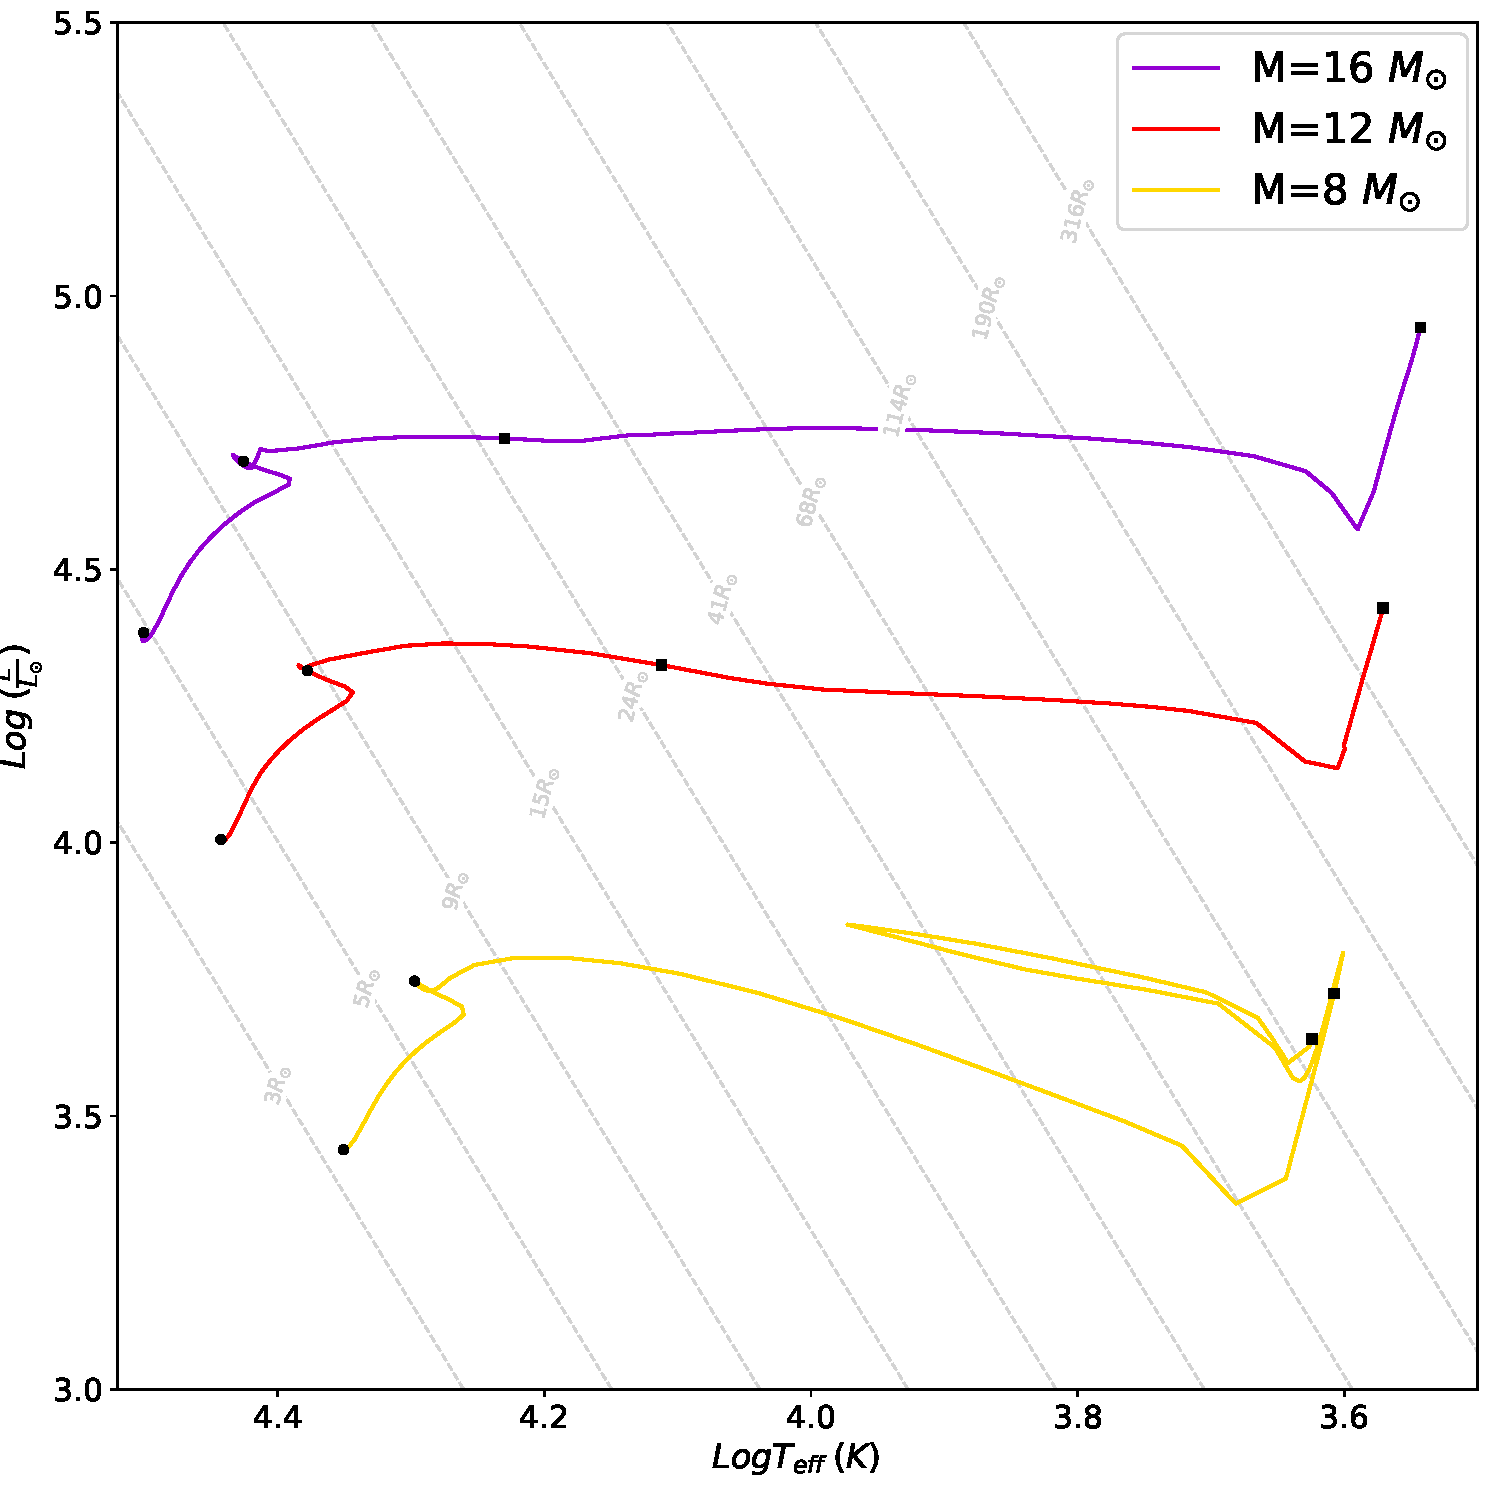
\includegraphics[width=0.9\textwidth]{Thesis/graphs/HR_massive_stars.pdf}
    \caption{Hertzsprung-Russell diagram. Evolutionary tracks for three stars with masses 8, 12 and 16 M$_{\odot}$ at solar metallicity until the end of Helium burning. Specific moments in the evolution of the stars are noted by black circles and squares as explained in the text. The tracks are calculated with MESA \citep{paxton2010modules,paxton2013modules,paxton2015modules,paxton2019modules}. The dashed lines show lines of constant radii by means of the Stefan–Boltzmann law.}
    \label{fig:HR_massive_stars}
\end{figure}
The Hertzsprung-Russell (HR) diagram in \cref{fig:HR_massive_stars} shows three evolutionary tracks for massive stars. The black circles correspond to the Zero Age Main Sequence (ZAMS) and the Terminal Age Main Sequence (TAMS). At ZAMS, the star having started the hydrogen burning in its core, achieves thermal equilibrium (TE), $L_{nuc}/L =1$, while TAMS is defined as the core hydrogen exhaustion point. Additionally, the black squares represent the start and end of helium burning in the core, respectively. In both cases the end of nuclear burning in the core is defined as the point when hydrogen and helium core mass fractions are $< 0.01$. The change in the star's physical radius occurs on different timescales depending on the physical mechanism buried beneath these processes. On nuclear timescale ($t_{nuc}$, see \eqref{eq:nuclear_timsecale}), stars evolve throughout the main sequence (MS) and the helium-burning phase, while on thermal timescale ($t_{th}$, see \eqref{eq:thermal_timsecale}), stars expand during the H-shell burning phase.

During the MS, hydrogen is fused into $^4$He. Independent of the ongoing reaction channel (pp or CNO), the luminosity of the star increases during this phase, (L$\,\propto\,\mu^{4}\,M^3$), due to the change in the core's composition ($\mu$ increases). Nevertheless, the way in which a star evolves through the MS-phase depends on its mass. Stars with masses M\,$\geq$\,1.3\,M$_\odot$, consequently massive stars too, are driven by the CNO-cycle ($\epsilon_{CNO}\,\propto\,\rho_{c}T^{18}_{c}$). The thermostatic action of the CNO-cycle causes the envelope to expand and, as a result, a decrease in effective temperature. Stars driven by the CNO-cycle evolve through larger radii and lower T$_{eff}$ than stars driven by the pp-cycle. Additionally, stars with masses M\,$\geq$\,1.3\,M$_\odot$ have convective cores, since the energy produced is too large to be transported by radiation ($\nabla_{rad} > \nabla_{ad}$). One effect of the convection on the evolution is that the MS-lifetime is extended (more detailed discussion in \cref{sub:mixing}). Another effect is that as the core approaches the end of H-burning, the reactions suddenly cease in the whole core, threatening the thermal equilibrium of the star. In response the temperature of the core needs to increase in order to keep the same energy generation rate leading to the contraction of the star. This is evident in the second part of the MS (see \cref{fig:HR_massive_stars}), where we observe the ``hook'' feature. 

At TAMS, where the hydrogen in the core has been depleted, hydrogen burning occurs in a shell around the core, while the central temperature is insufficient to initiate burning in the helium core. From that point on, the star enters the Hertzsprung gap branch and the evolution is driven by the mirror principle. The core contracts in $t_{th}$ in an attempt to reach thermal equilibrium, while the envelope expands. The aforementioned behavior is evident in Fig.\ref{fig:HR_massive_stars}, as the stars move towards bigger radius and lower effective temperature. An important thing to mention is that during this phase the temperature in the core is raising up and should not be confused with the effective temperature. Stars of less than $12$M$_{\odot}$ reach effective temperatures as low as ($10^{3.7}$K) 5000K before helium ignition. At this moment, they begin to ascend the red giant branch (RGB), which is accompanied by a significant rise in luminosity and radius. Due to the low effective temperature the opacity of the envelope rises and the latter becomes gradually convective. The prohibited zone of the HR-diagram is located to the right of the RGB, where hydrostatic equilibrium cannot be established. Any star in this zone will travel quickly towards the RGB. The red giant star has a compact core and an extensive envelope that extends hundreds of solar radii. When the temperature in the core exceeds $T_c \sim 10^8 K$, helium core burning begins, and the red giant phase ends. For stars with $M \geq 12$M$_{\odot}$, helium ignites before the effective temperature has dropped to a few thousand Kelvin. The stellar tracks for stars of less than $12$M$_{\odot}$ form a loop on the HR-diagram during helium burning, also known as the horizontal branch. The loop is accompanied by a drop and increase in the stellar radius. As the blazing front advances from the core to a shell enclosing the core, the star's outer layers expand again, and the evolution continues. For a more in depth description of the MS and post-MS evolution I direct the reader to \cite{pols2011stellar}.

\subsection{Stellar Winds}

Stellar winds play an important role in stellar evolution because they cause mass and angular momentum loss from the star. During the final stages of evolution on the AGB, low- and intermediate-mass stars experience significant mass-loss, which removes the remaining envelope, leaving only C-O white dwarfs as their final remnants \citep{marigo2007evolution}. On the other hand, for masses greater than 15 M$_{\odot}$, mass-loss by stellar winds becomes important during all evolution phases, including the main sequence. Observations in the ultraviolet and infrared spectrum show that these luminous massive stars experience rapid mass outflows (stellar winds) that can gradually erode their outer layers. For masses greater than 30 M$_{\odot}$, the mass-loss rates, $\dot{M}$, are so great that the mass-loss timescale, $t_{ml} = M / \dot{M}$, becomes shorter than the nuclear timescale, $t_{nuc}$. Even though stellar winds are fundamental in the formation and evolution of massive stars, the stellar wind mechanisms involved are not well understood in many cases. Hence $\dot{M}$ is frequently quite uncertain introducing significant uncertainties in the evolution of massive stars.

Driven by observations and theoretical models, stellar winds are usually in hot and cold winds because they are generated by different mechanisms. Numerous mass-loss rate prescriptions have been proposed, with $\dot{M}$ varying in different parts of the HR diagram. Hot, luminous massive stars (OB-type MS stars and blue supergiants, BSG) experience a stellar wind driven by radiation. Radiation pressure causes an outward acceleration at frequencies corresponding to absorption lines in the spectrum, where the interaction between photons and matter is strong. Because it is primarily the lines of the heavier elements that contribute to line driving, radiation-driven mass-loss is dependent also on metallicity \citep{vink2001mass}. Cool, luminous massive stars known as red supergiants (RSG) produce a stellar wind, which is likely caused by a combination of stellar pulsations and radiation pressure on dust particles that accumulate in the cool outer atmosphere, similarly with AGB stars. Because there are no theoretical predictions, empirical formulas that fit the average observed mass-loss rates of stars of roughly solar metallicity are used in theoretical studies. For example, mass-loss prescriptions based on \cite{reimers1975circumstellar,de1988mass,nieuwenhuijzen1990parametrization} are commonly used.

\subsection{Internal Mixing}\label{sub:mixing}

Even though the overall stellar evolution is only slightly affected by the initial chemical composition, a variety of internal mixing process can impact the life cycle, particularly of massive ($M>8$ M$_{\odot}$), stars \citep{langer2012presupernova}. Apart from convection, convective overshooting, semiconvection, and rotationally induced mixing are the most important internal mixing process \citep{schootemeijer2019constraining} and are still poorly understood. 

{\bf Convection}

{\bf Convective Overshooting}

Convective overshooting refers to the process of mixing beyond the boundaries of convective regions, which can occur when convective cells penetrate into radiative regions due to their non-zero velocity \citep{alongi1993evolutionary,brott2011rotating,schootemeijer2019constraining}. In stars with convective cores, e/g/ intermediate and massive stars, the size of the core is effectively enlarged through mechanisms such as convective core overshooting. This overshooting brings additional hydrogen into the core of the star and therefore directly impacts the final He core mass and main-sequence (MS) lifetime as well as the evolution of the stars after the MS.

{\bf Semiconvection}

{\bf Rotationally Induced Mixing}
